% file: algebra-without-dpsc_talk.tex
% created: 2013-08-13, 12:44:29 PM (-0500 CDT)

%=========================================================================={{{1
%\documentclass[compress]{beamer}
\documentclass[compress,handout]{beamer}
\usepackage{amsfonts,amsmath,amssymb,amsthm}
\usepackage{multirow, tabularx}
\usepackage{tikz, float}
\usetikzlibrary{calc,decorations.pathreplacing,matrix,arrows,positioning}

% color settings
\mode<presentation>{
\usetheme{Madrid}
\usecolortheme{default}
\beamertemplatenavigationsymbolsempty
}
\setbeamercolor{alerted text}{fg=blue}

% symbol definitions
\newcommand{\NN}{\mathbb{N}}
\newcommand{\ZZ}{\mathbb{Z}}
\newcommand{\QQ}{\mathbb{Q}}
\newcommand{\V}{\mathcal{V}}
\newcommand{\A}{\mathbb{A}}

% symbol overrides
\renewcommand{\phi}{\varphi}
\renewcommand{\epsilon}{\varepsilon}

% theorems and similar environments
\theoremstyle{plain} \newtheorem{thm}{Theorem}
\newtheorem{prop}[thm]{Proposition}
\newtheorem{lem}[thm]{Lemma}
\newtheorem{cor}[thm]{Corollary}
\theoremstyle{definition} \newtheorem{defn}[thm]{Definition}
\theoremstyle{remark} \newtheorem*{rk}{Remark}
\theoremstyle{plain} \newtheorem*{question}{Question}
\newtheorem*{conj}{Conjecture}

% custom commands
\newcommand{\mat}[1]{ \ensuremath{\begin{bmatrix} #1 \end{bmatrix}} }
\newcommand{\Case}[1]{\smallskip \textbf{Case #1:}}
\newcommand{\m}[1]{\mathbb{#1}}   % for models

% document specific stuff
\newcommand{\T}{\mathcal{T}}
\newcommand{\Cg}{\text{Cg}}
\newcommand{\Con}{\text{Con}}
%==========================================================================}}}1

%=========================================================================={{{1
\title[$\V(\A(\T))$ -- Two Counterexamples]{The Variety Generated by
$\A(\T)$ -- Two Counterexamples}
\author{Matthew Moore}
\institute[VU]{Vanderbilt University}
\date[2013-10-06]{October 6, 2013}
%==========================================================================}}}1

\begin{document} \maketitle

%==========================================================================={{{
\begin{frame} \frametitle{Park's Conjecture}
\begin{conj}[Park]
If $\V$ is a finitely generated variety with finite residual bound, then
$\V$ is finitely based.
\end{conj}

\pause \vspace{4ex}

Known if $\V$...
\begin{itemize}
  \item is congruence distributive (Baker).
  \pause \item is congruence modular (McKenzie).
  \pause \item is congruence meet-semidistributive (CSD($\wedge$)) (Willard).
  \pause \item has a difference term (Kearnes, Szendrei, Willard).
\end{itemize}
\end{frame}
%===========================================================================}}}

%==========================================================================={{{
\begin{frame} \frametitle{Finite Basis Theorems}
\uncover<1->{ \begin{thm}[Baker]
If $\V$ is a finitely generated congruence distributive variety, then $\V$
is finitely based.
\end{thm} }

\uncover<3->{ Some alternate proofs use:
\begin{itemize}
  \uncover<4->{ \item definable principal subcongruences }
  \uncover<5->{ \item bounded Maltsev depth }
\end{itemize} }

\uncover<2->{ \begin{thm}[Willard]
If $\V$ is a finitely generated congruence meet-semidistributive and has
finite residual bound, then $\V$ is finitely based.
\end{thm} }

\uncover<6->{ Do alternate proofs exist that use:
\begin{itemize}
  \item definable principal subcongruences?
  \item bounded Maltsev depth?
\end{itemize} }
\end{frame}
%===========================================================================}}}

%==========================================================================={{{
% question
\begin{frame}
\begin{question}
If $\A$ generates a variety that has finite residual bound and is
CSD($\wedge$), does the variety have...
\begin{itemize}
  \item definable principal subcongruences?
  \item bounded Maltsev depth?
\end{itemize}
\end{question}
\end{frame}
%===========================================================================}}}

%==========================================================================={{{
\begin{frame} \frametitle{Definable Principal Subcongruences}
\vspace{-2ex}
\begin{defn}
A variety $\V$ is said to have \emph{definable principal subcongruences
(DPSC)} if there are congruence formulas
$\Gamma(\text{-},\text{-},\text{-},\text{-})$ and
$\psi(\text{-},\text{-},\text{-},\text{-})$ such that for all $\A\in \V$ and
all $a,b\in A$ there exist $c,d\in A$ such that $\Gamma(c,d,a,b)$ witnesses
$(c,d)\in \Cg^{\A}(a,b)$ and $\psi(-,-,c,d)$ defines $\Cg^{\A}(c,d)$.
\end{defn}

\vfill

\begin{columns}
\begin{column}{0.37\textwidth}
  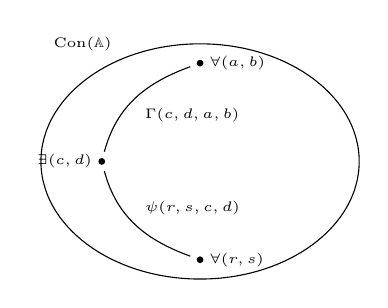
\begin{tikzpicture}[font=\tiny,smooth,linelab/.style={fill=white,inner sep=0.1em}]
    \node (ab) {};
    \node (cd) [below left=of ab] {};
    \node (rs) [below right=of cd] {};

    \filldraw (ab) node[right]{$\forall (a,b)$} circle (0.1em)
      (cd) node[left]{$\exists (c,d)$} circle (0.1em)
      (rs) node[right]{$\forall (r,s)$} circle (0.1em);

    \draw (ab) to[out=200,in=75] node[below right]{$\Gamma(c,d,a,b)$} (cd)
      (cd) to[out=-75,in=-200] node[above right]{$\psi(r,s,c,d)$} (rs);

    \coordinate (c) at ($0.5*(ab)+0.5*(rs)$);
    \coordinate (t) at ($(c)+(0,4.25em)$);
    \node [left=of t] {$\Con(\A)$};
    \draw (c) ellipse (5.75em and 4.25em);
  \end{tikzpicture}
\end{column}

\pause

\begin{column}{0.63\textwidth}
If $\V$ has DPSC and $\Cg^{\A}(a,b)$ is an atomic congruence of some $\A\in
\V$, then $\psi(-,-,a,b)$ defines $\Cg^{\A}(a,b)$.
\end{column}
\end{columns}
\end{frame}
%===========================================================================}}}

%==========================================================================={{{
\begin{frame} \frametitle{Definable Principal Subcongruences}
If $\V$ has DPSC, then every atomic congruence is defined by $\psi$.

\pause \vspace{6ex}

This means...
\begin{itemize} \setlength{\itemsep}{4ex}
  \item there is $N\in \NN$ such that 
  \begin{itemize}
    \pause \item for all $\A\in \V$,
    \pause \item all $a,b\in A$ with $\Cg^{\A}(a,b)$ atomic, and 
    \pause \item all $(c,d)\in \Cg^{\A}(a,b)$
  \end{itemize}
  \pause there is $\m{B}\leq \A$ of size at most $N$ with $(c,d)\in
  \Cg^{\m{B}}(a,b)$.

  \pause \item to disprove DPSC for $\V$, find $\A\in \V$ and atomic
  $\Cg^{\A}(a,b)$ such that there is no bound on minimal $\m{B}\leq \A$
  witnessing $(c,d)\in \Cg^{\m{B}}(a,b)$.
\end{itemize}
\end{frame}
%===========================================================================}}}

%==========================================================================={{{
\begin{frame} \frametitle{Bounded Maltsev Depth}
\begin{defn}
A variety $\V$ has \emph{Maltsev depth $N$} if for every $\A\in \V$ and
every $a,b \in \A$, $(c,d)\in \Cg^{\A}(a,b)$ is witnessed by a Maltsev chain
with associated polynomials of compositional depth at most $N$ (and $N$ is
minimal).
\end{defn}

\vspace{4ex}

\begin{columns}
\begin{column}{0.5\textwidth}
  \centering
  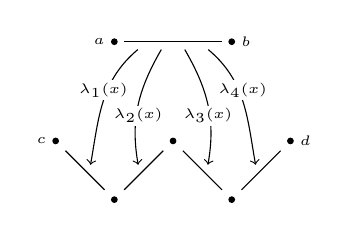
\begin{tikzpicture}
    [font=\tiny,smooth,linelab/.style={fill=white,inner sep=0.1em}]
    \begin{scope}[node distance=2em]
      \node (c) {};
      \node (c1) [below right=of c] {};
      \node (c2) [above right=of c1] {};
      \node (c3) [below right=of c2] {};
      \node (d) [above right=of c3] {};
    \end{scope}
    \node (a) [above=5em of c1] {};
    \node (b) [above=5em of c3] {};

    \foreach \n in {a,b,c,c1,c2,c3,d} {
      \filldraw (\n) circle (0.1em);
    }
    \node at (a) [left] {$a$};
    \node at (b) [right] {$b$};
    \node at (c) [left] {$c$};
    \node at (d) [right] {$d$};
    \foreach \n / \m in {a/b,c/c1,c1/c2,c2/c3,c3/d} {
      \draw (\n) -- (\m);
    }
    \draw[->] ($0.8*(a)+0.2*(b)+(0,-0.1)$) to[out=220,in=80] 
      node[linelab,above]{$\lambda_1(x)$} ($0.5*(c)+0.5*(c1)+(0.07,0.07)$);
    \draw[->] ($0.6*(a)+0.4*(b)+(0,-0.1)$) to[out=240,in=100] 
      node[linelab,below]{$\lambda_2(x)$} ($0.5*(c1)+0.5*(c2)+(-0.07,0.07)$);
    \draw[->] ($0.4*(a)+0.6*(b)+(0,-0.1)$) to[out=300,in=80] 
      node[linelab,below]{$\lambda_3(x)$} ($0.5*(c2)+0.5*(c3)+(0.07,0.07)$);
    \draw[->] ($0.2*(a)+0.8*(b)+(0,-0.1)$) to[out=320,in=100] 
      node[linelab,above]{$\lambda_4(x)$} ($0.5*(c3)+0.5*(d)+(-0.07,0.07)$);
  \end{tikzpicture}
\end{column}

\begin{column}{0.5\textwidth}
$\forall \A\in \V$, $\forall a,b,c,d\in A$...

\vspace{2ex}

$\lambda_i(x)$ has uniformly bounded depth.
\end{column}
\end{columns}

\end{frame}
%===========================================================================}}}

%==========================================================================={{{
\begin{frame} \frametitle{The Strategy}
\begin{itemize} \setlength{\itemsep}{4ex}
  \item Find $\V$ that is CSD($\wedge$) and has finite residual bound.

  \pause \item Find family of $\m{B}_n\in \V$ and $a,b,b_n,c_n\in B_n$ such
  that...
  \begin{columns} \begin{column}{0.4\textwidth}
      \centering
      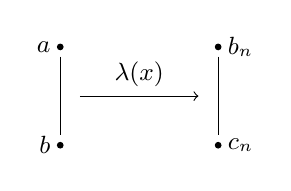
\begin{tikzpicture}[font=\small,smooth]
        \node (a) {};
        \node (0) [below=of a] {};
        \node (b) [right=5em of a] {};
        \node (c) [below=of b] {};

        \foreach \n in {a,0,b,c} {
          \filldraw (\n) circle (0.1em);
        }
        \draw (a) -- (0) (b) -- (c);
        \node at (a) [left] {$a$};
        \node at (0) [left] {$b$};
        \node at (b) [right] {$b_n$};
        \node at (c) [right] {$c_n$};
        \draw[->] ($0.5*(a)+0.5*(0)+(0.25,0)$) -- 
          node[above]{$\lambda(x)$} ($0.5*(b)+0.5*(c)+(-0.25,0)$);
      \end{tikzpicture}
    \end{column} \begin{column}{0.6\textwidth}
      \begin{itemize}
        \item $\Cg^{\m{B}_n}(a,b)$ is atomic.

        \pause \item This is the ``best'' Maltsev chain witnessing
        $(b_n,c_n)\in Cg^{\m{B}}(a,b)$.

        \pause \item The number of parameters used in $\lambda(x)$ scales
        with $n$.

        \pause \item $\lambda(x)$ has depth that scales with $n$.
      \end{itemize}
    \end{column} \end{columns}

  \pause \item Letting $n$ grow will demonstrate that $\V$ has neither DPSC
  nor bounded Maltsev depth.
\end{itemize}
\end{frame}
%===========================================================================}}}

%==========================================================================={{{
\begin{frame} \frametitle{The Algebra $\A(\T)$}
\begin{itemize}\setlength{\itemsep}{4ex}
  \item McKenzie associated to each Turing machine $\T$ an algebra $\A(\T)$
  such that $\V(\A(\T))$ has finite residual bound iff $\T$ halts.

  \pause \item $\A(\T)$ has a semilattice operation, so $\V(\A(\T))$ is
  CSD($\wedge$). \pause When $\T$ halts, $\V(\A(\T))$ has finite residual
  bound.

  \pause \item Willard proved that $\V(\A(\T))$ is finitely axiomatizable
  iff $\T$ halts.

  \pause \item By adding another operation to $\A(\T)$, I proved that
  $\V(\A'(\T))$ has DPSC iff $\T$ halts.

  \pause \item Is $\V(\A(\T))$ a counterexample to the claim that all such
  algebras have DPSC? \pause (\alert{Yes})
\end{itemize}
\end{frame}
%===========================================================================}}}

%==========================================================================={{{
\begin{frame} \frametitle{$\A(\T)$}
For a Turing machine $\T$ with $n$ states, the underlying set of $\A'(\T)$
has $(20n + 8)$ elements:
\begin{multline*}
  A'(\T) = \left\{ 0,1,2,H,C,D,\partial C, \partial D, \right. \\
  \left. C_{ir}^s, D_{ir}^s, M_i^r, \partial C_{ir}^s, \partial D_{ir}^s, 
    \partial M_i^r \mid 0\leq i\leq n \text{ and } r,s\in \{0,1\} \right\}.
\end{multline*}

\pause

$\A'(\T)$ has operations to emulate computation on certain tuples of the
indexed elements: \pause
\begin{align*}
  & \mathcal{L} = \left\{ L_{irt} \mid \T \text{ has instruction }
    (\mu_i,r,s,L,\mu_j) \text{ and } t\in \{0,1\} \right\}, \\
  & \mathcal{R} = \left\{ R_{irt} \mid \T \text{ has instruction }
    (\mu_i,r,s,R,\mu_j) \text{ and } t\in \{0,1\} \right\}.
\end{align*}

\pause

The operations of $\A(\T)$ are
\[
  \left\{ 0, \wedge, (\cdot), J, J', S_0, S_1, S_2, T, I, F, U_F^0, U_F^1
  \mid F\in \mathcal{L}\cup \mathcal{R} \right\}.
\]

\pause 

The algebra $\A'(\T)$ (has DPSC iff $\T$ halts) includes an operation $K$.
\end{frame}
%===========================================================================}}}

%==========================================================================={{{
% DPSC undec theorem
\begin{frame}
Let $\A'(\T)$ be $\A(\T)$ with a new operation, $K$, added to the language.

\begin{thm}
The following are equivalent:
\begin{itemize}
  \item $\T$ halts.
  \item $\V(\A'(\T))$ has finitely many SI's, all finite.
  \item $\V(\A'(\T))$ has DPSC.
  \item $\V(\A'(\T))$ is finitely axiomatizable.
\end{itemize}
\end{thm}

\pause

Proof involves analysis of Maltsev chains:
\begin{center} \begin{tikzpicture}[font=\small,smooth]
  \node (r1) {};
  \node (r2) [below=1.25em of r1] {};
  \foreach \i in {1,2} {
    \filldraw (r\i) circle (0.1em);
  }
  \draw (r1) -- node[left]{\tiny $F(\dots)$} (r2);

  \uncover<3->{
  \node (r5) at ($0.5*(r1)+0.5*(r2)$) [xshift=6em] {};
  \node (r4) [above=1.5em of r5] {};
  \node (r3) [above=1.5em of r4] {};
  \node (r6) [below=1.5em of r5] {};
  \node (r7) [below=1.5em of r6] {};
  \node (implies) at (r1|-r5) [xshift=3em] {$\Rightarrow$};
  \foreach \i in {3,...,7} {
    \filldraw (r\i) circle (0.1em);
  }
  \draw (r3) -- node[right]{\tiny $J'(\dots)$} (r4)
    (r4) -- node[right]{\tiny $J(\dots)$} (r5)
    (r5) -- node[right]{\tiny $J'(\dots)$} (r6)
    (r6) -- node[right]{\tiny $J'(\dots)$} (r7);
  }

  \uncover<4->{
  \node (r9) at (r5) [xshift=8em] {};
  \node (r8) [above=1.5em of r9] {};
  \node (r10) [below=1.5em of r9] {};
  \node (implies) at (r5) [xshift=5em] {$\Rightarrow$};
  \foreach \i in {8,9,10} {
    \filldraw (r\i) circle (0.1em);
  }
  \draw (r8) -- node[right]{\tiny $J'(\dots)$} (r9)
    (r9) -- node[right]{\tiny $J(\dots)$} (r10);
  }
\end{tikzpicture} \end{center}



\end{frame}
%===========================================================================}}}

%==========================================================================={{{
\begin{frame} \frametitle{The Counterexample}
Define $\m{B}_n = \left<\left\{a,b_i,d_i \mid 2\leq i\leq n\right\} \right>$
where
\vspace{-1ex}
\begin{center} \footnotesize $\begin{aligned}
  b_i & = (D,D,\ldots, \stackrel{i}{\hat{D}},0,\ldots,0), & 
    a & = b_1, \\
  d_i & = (D,\ldots,D,\stackrel{i}{\hat{\partial D}},0,\ldots,0), &
    c_i & = (0,D,\ldots,\stackrel{i}{\hat{D}},0,\ldots,0).
\end{aligned}$ \end{center}

\pause

$\A(\T)$ has \textbf{lots} of operations, but the only nonzero ones on
$\m{B}_n$ are
\begin{center} \footnotesize $\begin{aligned}
  \uncover<3->{ 
  x\wedge y & = \begin{cases} 
    x & \text{if } x=y \\
    0 & \text{otherwise}
  \end{cases} } &
  \uncover<4->{
  S_2(u,v,x,y,z) & = \begin{cases}
    (x\wedge y) \vee (x\wedge z) & \text{if } u = \partial v \\
    0                            & \text{otherwise}
  \end{cases} } \\
  \uncover<5->{ 
  J(x,y,z) & = \begin{cases} 
    x         & \text{if } x = y \\
    x\wedge z & \text{if } x = \partial y \\
    0         & \text{otherwise}
  \end{cases} } &
  \uncover<6->{
  J'(x,y,z) & = \begin{cases} 
    x\wedge z & \text{if } x = y \\
    x & \text{if } x = \partial y \\
    0 & \text{otherwise}
  \end{cases} }
\end{aligned}$ \end{center}

\uncover<7->{ 
Look at $(b_n,d_n)\in \Cg^{\m{B}_n}(a,0)$.
}

%\begin{center} \begin{tikzpicture}[font=\small,smooth,node distance=3em]
%  \node (a) {$a$};
%  \node (0) [below=of a] {$0$};
%  \node (b2) [right=of a] {$b_2$};
%  \node (c2) [below=of b2] {$c_2$};
%  \node (b3) [right=of b2] {$b_3$};
%  \node (c3) [below=of b3] {$c_3$};
%  \node (dots) at ($0.5*(b3)+0.5*(c3)$) [right,xshift=1.25em] {$\cdots$};
%  \node (bn) [right=2.75em of b3] {$b_n$};
%  \node (cn) [below=of bn] {$c_n$};
%
%  \foreach \n / \m in {a/0,b2/c2,b3/c3,bn/cn} {
%    \draw (\n) -- (\m);
%  }
%  \draw[->] ($0.5*(a)+0.5*(0)+(0.1,0)$) 
%    -- node[above]{\tiny $J'(b_2,d_2,x)$} ($0.5*(b2)+0.5*(c2)+(-0.1,0)$);
%  \draw[->] ($0.5*(b2)+0.5*(c2)+(0.1,0)$) 
%    -- node[above]{\tiny $J'(b_3,d_3,x)$} ($0.5*(b3)+0.5*(c3)+(-0.1,0)$);
%
%  \draw[->] ($0.5*(b3)+0.5*(c3)+(0.1,0)$) -- (dots);
%  \draw[->] ($(dots)+(0.3,0)$) -- ($0.5*(bn)+0.5*(cn)+(-0.1,0)$);
%
%  \coordinate (t1) at ($(0)+(-0.1,-0.5)$);
%  \draw ($0.5*(a)+0.5*(0)+(-0.1,0)$) to[out=180,in=180] (t1);
%  \coordinate (t2) at ($(cn)+(0.1,-0.5)$);
%  \draw (t1) -- node[below]{\tiny$J'(b_n,d_n,J'(b_{n-1},d_{n-1},\cdots
%  J(b_2,d_2,x)\cdots ))$} (t2);
%  \draw[->] (t2) to[out=0,in=0] ($0.5*(bn)+0.5*(cn)+(0.1,0)$);
%\end{tikzpicture} \end{center}
\end{frame}
%===========================================================================}}}

%==========================================================================={{{
\begin{frame} \frametitle{The Calculation}
\begin{center} 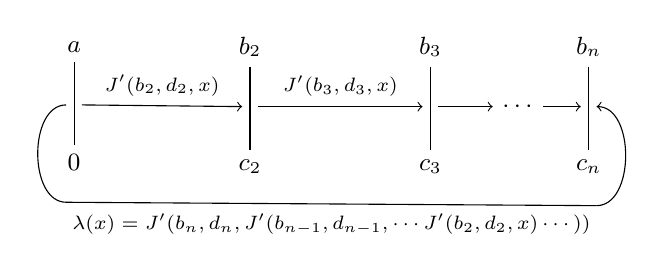
\begin{tikzpicture}[font=\small,smooth,node distance=3em]
  \node (a) {$a$};
  \node (0) [below=of a] {$0$};
  \node (b2) [right=5em of a] {$b_2$};
  \node (c2) [below=of b2] {$c_2$};
  \node (b3) [right=5em of b2] {$b_3$};
  \node (c3) [below=of b3] {$c_3$};
  \node (dots) at ($0.5*(b3)+0.5*(c3)$) [right,xshift=2.25em] {$\cdots$};
  \node (bn) [right=4.15em of b3] {$b_n$};
  \node (cn) [below=of bn] {$c_n$};

  \foreach \n / \m in {a/0,b2/c2,b3/c3,bn/cn} {
    \draw (\n) -- (\m);
  }
  \draw[->] ($0.5*(a)+0.5*(0)+(0.1,0)$) 
    -- node[above]{\scriptsize $J'(b_2,d_2,x)$} ($0.5*(b2)+0.5*(c2)+(-0.1,0)$);
  \draw[->] ($0.5*(b2)+0.5*(c2)+(0.1,0)$) 
    -- node[above]{\scriptsize $J'(b_3,d_3,x)$} ($0.5*(b3)+0.5*(c3)+(-0.1,0)$);

  \draw[->] ($0.5*(b3)+0.5*(c3)+(0.1,0)$) -- (dots);
  \draw[->] ($(dots)+(0.3,0)$) -- ($0.5*(bn)+0.5*(cn)+(-0.1,0)$);

  \coordinate (t1) at ($(0)+(-0.1,-0.5)$);
  \draw ($0.5*(a)+0.5*(0)+(-0.1,0)$) to[out=180,in=180] (t1);
  \coordinate (t2) at ($(cn)+(0.1,-0.5)$);
  \draw (t1) -- node[below]{\scriptsize $\lambda(x) =
  J'(b_n,d_n,J'(b_{n-1},d_{n-1},\cdots J'(b_2,d_2,x)\cdots ))$} (t2);
  \draw[->] (t2) to[out=0,in=0] ($0.5*(bn)+0.5*(cn)+(0.1,0)$);
\end{tikzpicture} \end{center}

\begin{itemize} \setlength{\itemsep}{4ex}
  \pause \item $\lambda(x)$ uses $2(n-1)$ distinct parameters (so the
  smallest $\m{B}\leq \m{B}_n$ witnessing $(b_n,c_n)\in \Cg^{\m{B}_n}(0,a)$
  is of size $\geq 2(n-1)$). \\
  \pause \alert{Therefore $\V(\A(\T))$ doesn't have DPSC.}

  \pause \item The compositional depth of $\lambda(x)$ is $n-1$. \\
  \pause \alert{Therefore $\V(\A(\T))$ doesn't have bounded Maltsev depth.}
\end{itemize}
\end{frame}
%===========================================================================}}}

%==========================================================================={{{
\begin{frame} \frametitle{What about the $K$ operation?}
\uncover<2-|handout:1>{
With $K$ in the language, $\m{B}_n$ contains an element $p$ such that...
}

\begin{center} 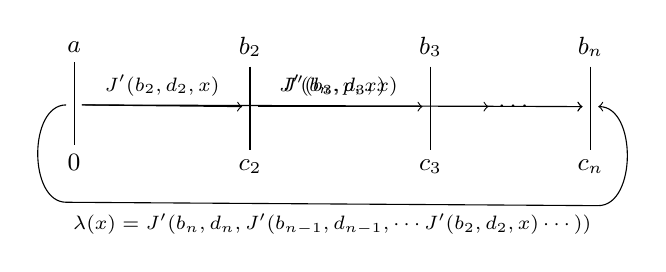
\begin{tikzpicture}[font=\small,smooth,node distance=3em]
  \node (a) {$a$};
  \node (0) [below=of a] {$0$};

  \uncover<-1|handout:0>{
  \node (b2) [right=5em of a] {$b_2$};
  \node (c2) [below=of b2] {$c_2$};
  \node (b3) [right=5em of b2] {$b_3$};
  \node (c3) [below=of b3] {$c_3$};
  \node (dots) at ($0.5*(b3)+0.5*(c3)$) [right,xshift=2.1em] {$\cdots$};
  }

  \node (bn) [right=17.25em of a] {$b_n$};
  \node (cn) [below=of bn] {$c_n$};

  \draw (a) -- (0);
  \draw (bn) -- (cn);

  \uncover<-1|handout:0>{
  \draw (b2) -- (c2);
  \draw (b3) -- (c3);
  \draw[->] ($0.5*(a)+0.5*(0)+(0.1,0)$) 
    -- node[above]{\scriptsize $J'(b_2,d_2,x)$} ($0.5*(b2)+0.5*(c2)+(-0.1,0)$);
  \draw[->] ($0.5*(b2)+0.5*(c2)+(0.1,0)$) 
    -- node[above]{\scriptsize $J'(b_3,d_3,x)$} ($0.5*(b3)+0.5*(c3)+(-0.1,0)$);

  \draw[->] ($0.5*(b3)+0.5*(c3)+(0.1,0)$) -- (dots);
  \draw[->] ($(dots)+(0.3,0)$) -- ($0.5*(bn)+0.5*(cn)+(-0.1,0)$);
  }

  \coordinate (t1) at ($(0)+(-0.1,-0.5)$);
  \draw ($0.5*(a)+0.5*(0)+(-0.1,0)$) to[out=180,in=180] (t1);
  \coordinate (t2) at ($(cn)+(0.1,-0.5)$);
  \draw (t1) -- node[below]{\scriptsize $\lambda(x) =
  J'(b_n,d_n,J'(b_{n-1},d_{n-1},\cdots J'(b_2,d_2,x)\cdots ))$} (t2);
  \draw[->] (t2) to[out=0,in=0] ($0.5*(bn)+0.5*(cn)+(0.1,0)$);

  \uncover<2-|handout:1>{
  \draw[->] ($0.5*(a)+0.5*(0)+(0.1,0)$) 
    -- node[above]{\scriptsize $J'(b_n,p,x)$} ($0.5*(bn)+0.5*(cn)+(-0.1,0)$);
  }
\end{tikzpicture} \end{center}

\uncover<3->{
The $K$ operation was introduced precisely so that things like $\lambda(x)$
could be simplified.
}
\end{frame}
%===========================================================================}}}

%==========================================================================={{{
\begin{frame} % thanks for all the fish
\centering \vfill
Thank you.
\vfill
\end{frame}
%===========================================================================}}}
\end{document}


